\chapter{Backbone}
The main controller of the application is the backbone, it is made by theAapi, and after its construction, it starts its own thread and takes control of the network library.

\subsection{The backbone class}
The backbone class controls the overall flow of the system by repeatedly checking the state of all buffers and deciding which buffer needs attention, if more than two buffers have accumulated a sufficient amount of data, it is up to the backbone to choose the most urgent of the two buffers to work with.

The end user application, does not decide how the backbone is allocated explicitly, instead, it will be created upon loading the library and instantiating the API layer. This means that the startup of the library implicitly will be part of the facade pattern.
The backbone class is also responsible for creation of the buffers and for handling settings and errors. The sizes of the buffers may be exposed through the API layer, for the end user to explicitly define buffer sizes, but the library should contain good default values, so the user does not need to configure this manually under most circumstances.

To prevent stalling other processes in the user application, the backbone runs in a separate thread. This introduces concurrency problems at the API layer, when the user application wishes to send and retrieve a message data may be lost, therefore the buffer must be constructed with a way to handle this situation, as this is outside the scope of the backbone itself.
The same can happen at the physical layer, but it is not the responsibility of the backbone or bufferclass to handle this.

Each of the buffers have an associated minimum and maximum value. Together with their size and datacount, they define the response of the backbone when there are borderline congestion.
The minimum value of a buffer is meant as a count of units that the system should aim to have in that buffer, when possible. For instance the physical layer buffer needs to have above a certain amount of frames ready to play, because the library cannot guarentee when it can expect to execute next. Therefore the more data there is in the output buffers, the longer the network thread can wait before executing agian.
The maximum value indicates how much data there can be in a buffer before the system is close to congestion. Therefore whenever there is too much data in a buffer, the backbone should prioritize moving it out.
Too much outgoing data, or too little ingoing data in the system buffers, does not represent a stability threat, and the library will continue to operate at full, or close to fullcapacity under these circumstances, this means that the minimum threshold values doesnt apply to ingoing buffers, and maximum threshold values doesnt apply to outgoing buffers.



The method for determining which buffer to work with, is based on the following criteria:

In the case of sending messages, the physical layer buffer should never be empty unless all the other buffers are empty, otherwise there will be unnecessary gaps in the audio output. This means that it is of high priority to move frames from the datalink layer to the physical layer.
At the same time, there must never be to many frames in the physical input buffer, otherwise data will be lost. Because buffer problems with the physical layer directly will result in erroronious operation of the library, these buffers must have the highest priority, when deciding where to "work". The inbound buffers has the highes priority, since faults here cause data loss, where as the other merely causes delays.

Next we have the data link buffers since, by the same logic, these can create congestion when there are to many frames to decode, which will later stall the physical layer, these will have high priority, but lower than the physical layer.
And again the outgoing data link buffers will create a lack of frames if they dont deliver decoded packages.

The same argument goes for the transport layer, which ofcourse has the lowest priority value.
 In the end the final priority queue is:

\begin{enumerate}
\item If amount of input frames > input frame maximum value, move frames from the physical layer.
\item If amount of output frames < output frames minimum value, move frames to the physical layer.
\item If amount of frames > frame maximum value, decode frames (produces inbound packages).
\item If amount of frames < frame minimum value, encode packages(produces outbound frames).
\item If amount of packages > package maximum value, decode packages(produces finished inbound messages).
\item If amount of packages < package minimum value, encode messages(produces outbound packages).
\end{enumerate}
This prioritized flow see figure \ref{fig:backboneprime} will ideally ensure that the system strives to stay in a "stable" state, during medium load time.
When the system is a bit more relaxed, that is, all values are within working parameters, the system will assign work in a way that reminds somewhat of round robin, that the system checks all buffers once, and then if there is no work to be done, goes to sleep for a predetermined amount of time. The starting buffer to check, is advanced through the six buffers for each attempt at general work, in accordance with flow \ref{fig:backboneGeneral}.

\subsection{The buffer class}


Since too much data in the outgoing buffers is untreatable (we cant give the data back to the user, and the audio wont play faster) with fixed size buffers, a mechanism is needed


To ensure maximum reuse of code a generalized buffer class is developed. This class provides one buffer for downwards data and one for upwards. Each buffer is a two-dimensional circular buffer provided by the included boost library. The buffer class contains methods for calling the layers and for providing information to the backbone.
By making the buffer two dimensional, it is possible to apply locks to individual sections of the data instead of a complete read/write lock, and thereby vastly increasing insert/delete operations.

Three  buffer objects are instantiated: A package buffer, a datagram buffer and a frame buffer. Each buffer is accessible from both the overlying and the underlying layer. And when a buffer is attended by the backbone it calls the appropriate function in the responsible layer.










\begin{figure}[htb]
	\begin{center}
	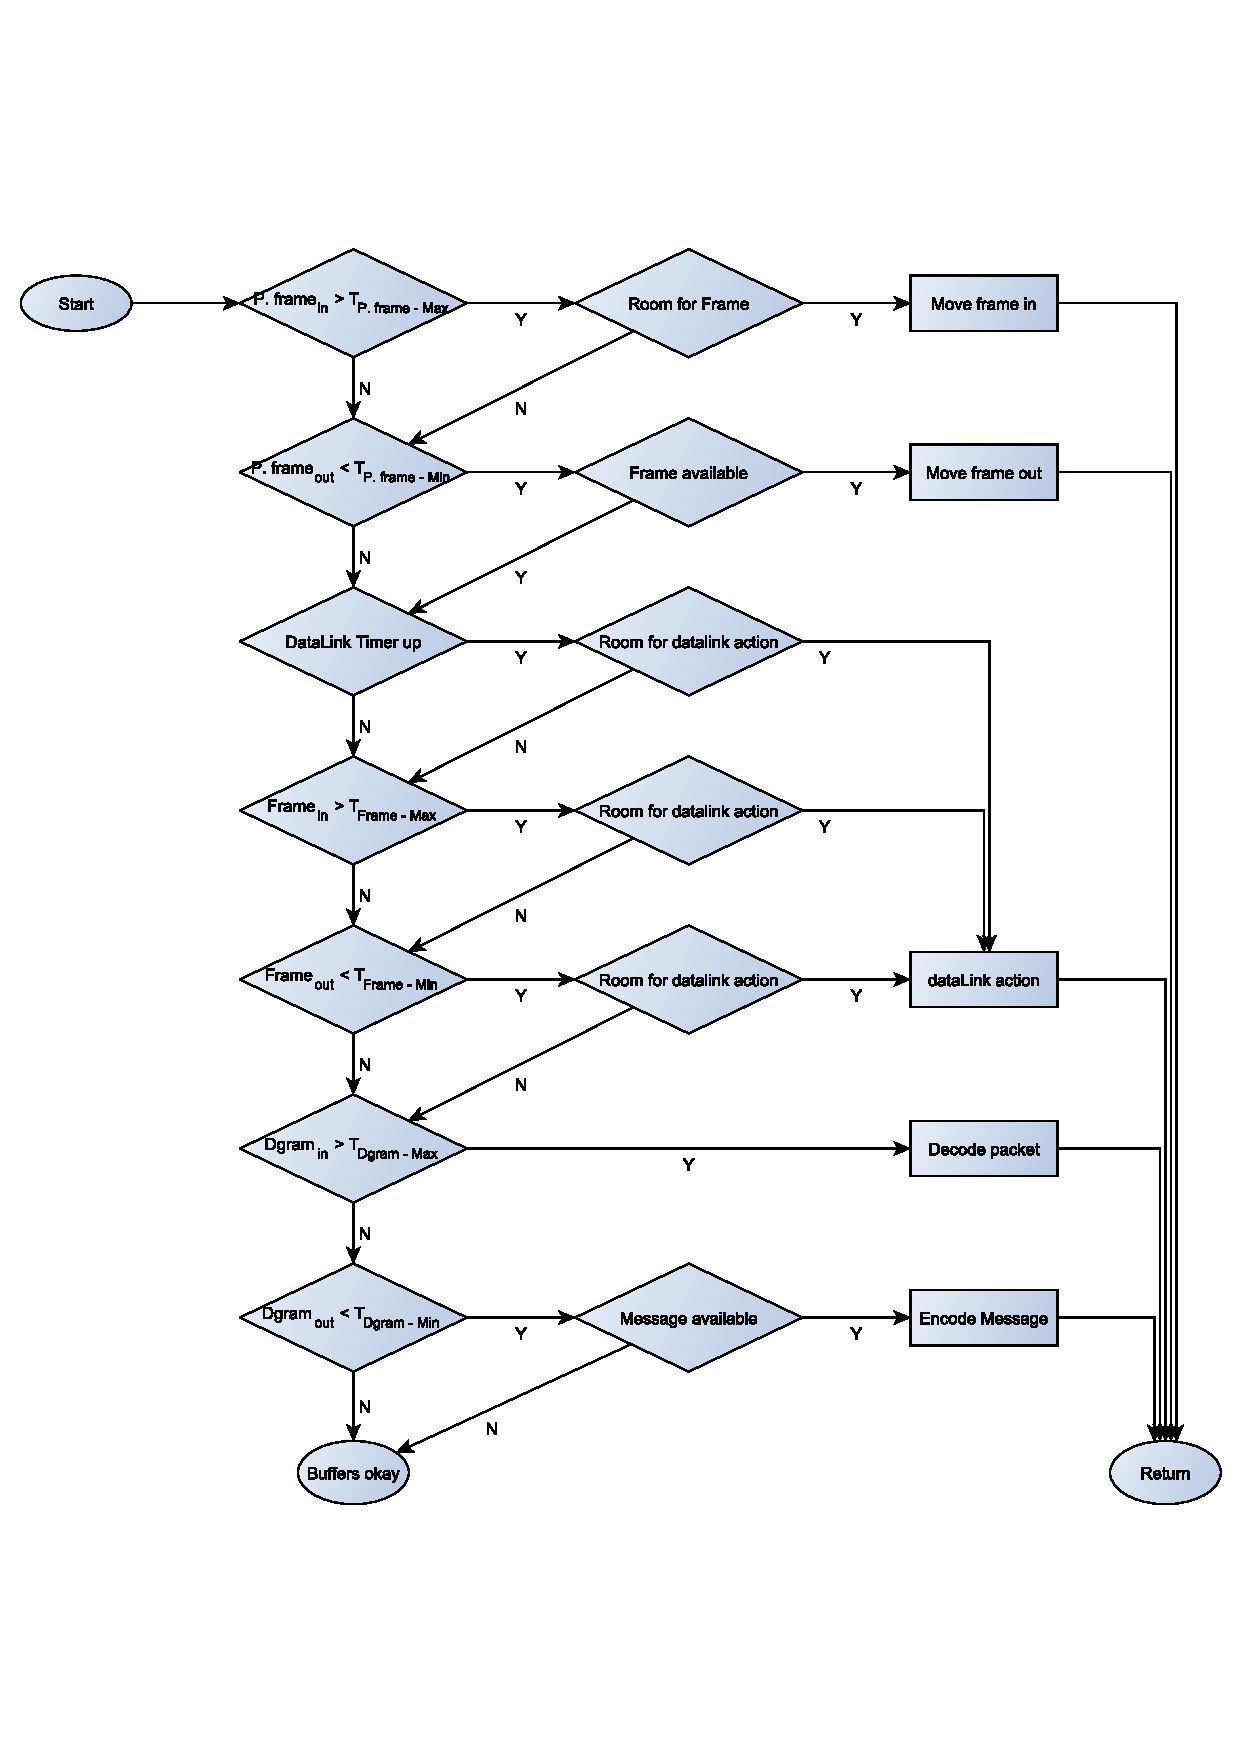
\includegraphics[scale=0.5,trim=0 0 0 0]{backbonePrime.pdf}
	\caption{Backbone primary flow}
	\label{fig:backboneprime}	
	\end{center}
\end{figure}


\begin{figure}[htb]
	\begin{center}
	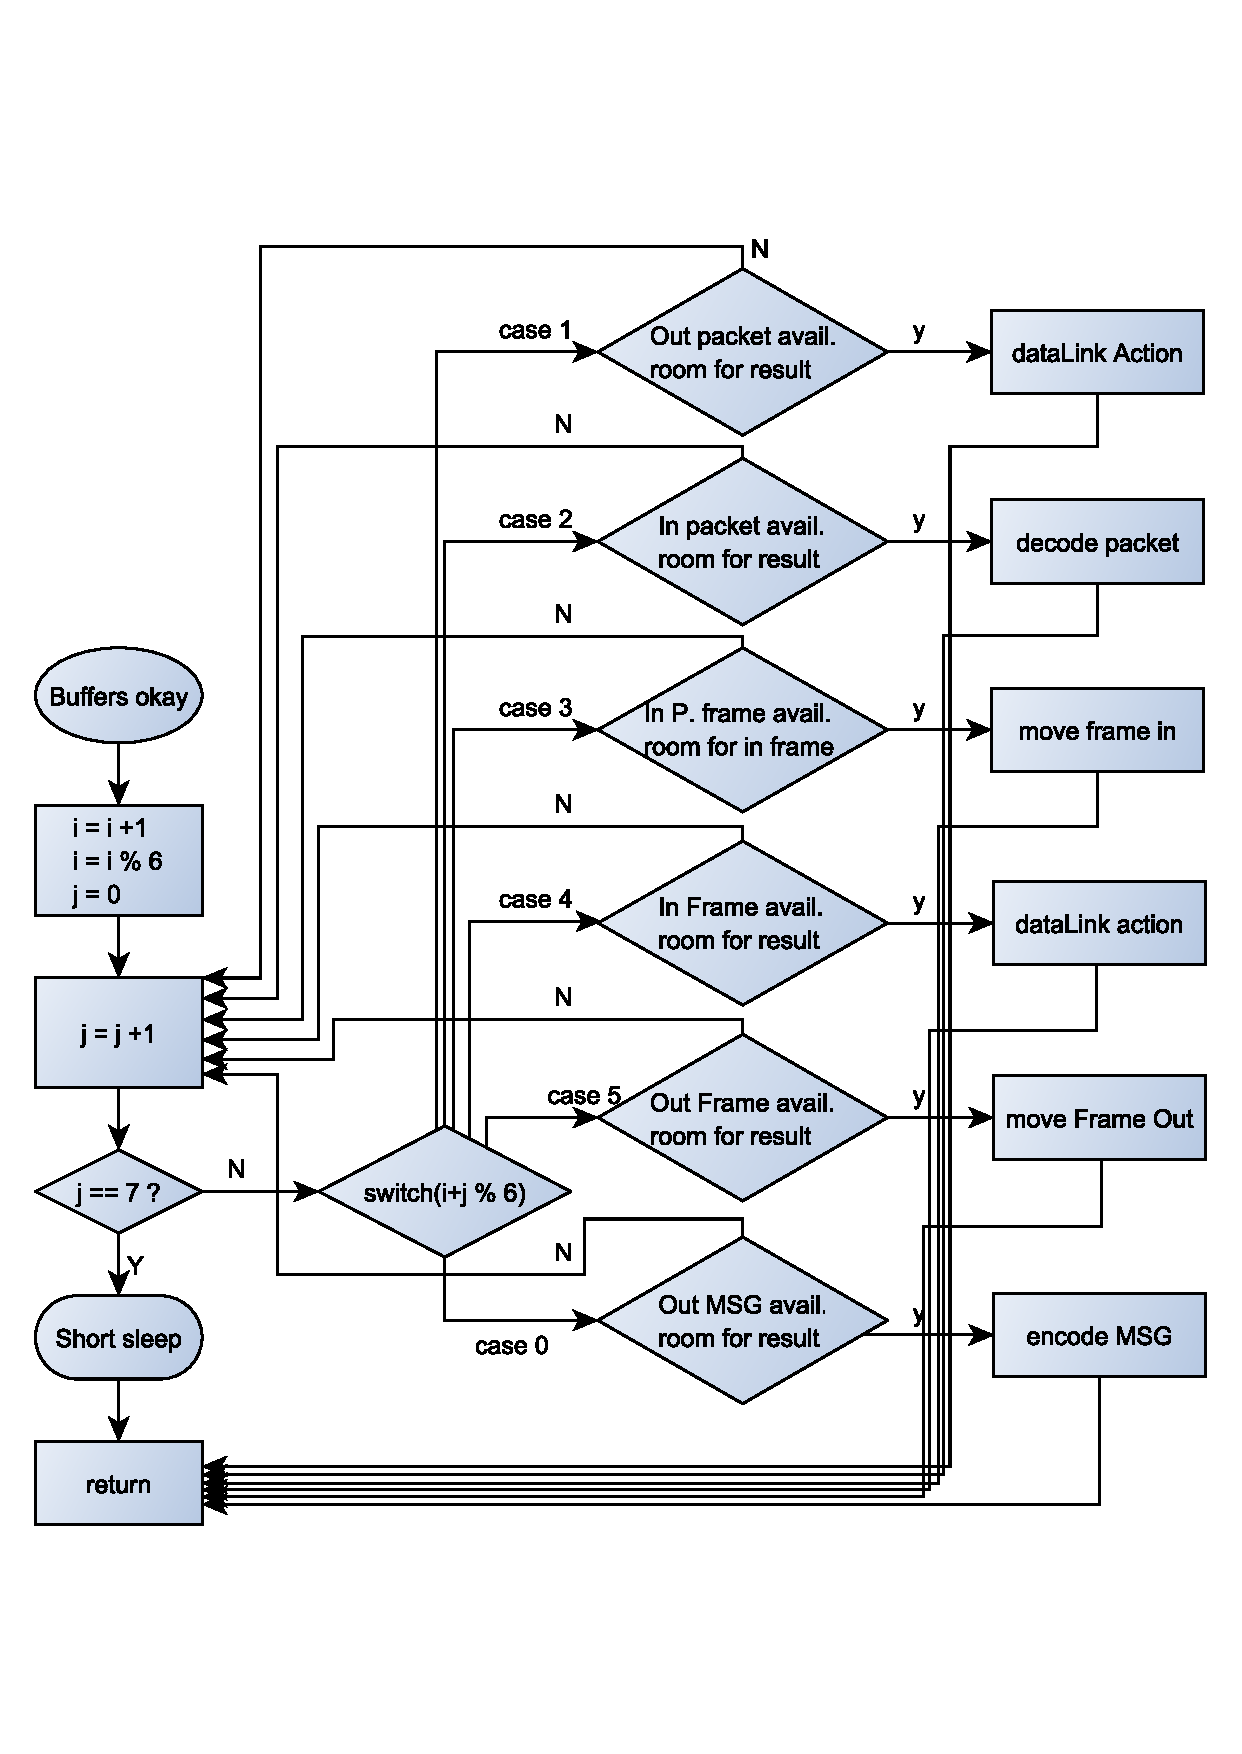
\includegraphics[scale=0.5,trim=0 0 0 0]{backboneGeneral.pdf}
	\caption{Backbone general flow)}
	\label{fig:backbonegeneralt}	
	\end{center}
\end{figure}
